




\newpage

\section{Zeitlich veränderliches Magnetfeld}

\subsection{Induktion}

Bis jetzt haben wir elektrische und magnetische Grössen angeschaut, die sich Zeitlich nicht ändern. \\
Sind beide Grössen konstant, so beeinflussen sie sich nicht. \\
Sobald sich jedoch der Magnetische Fluss $\phi$  \textbf{zeitlich ändert}, besteht einen Zusammenhang zwischen Magnetfeld und elektrischem Feld. \\
Wie magnetischer Fluss und Elektrisches Feld zusammenhängen beschreibt das \textbf{Induktionsgesetz}


\gl{Gleichung}{Induktionsgesetz}
\begingl
\formulaBegin
  $\displaystyle \oint_s \vec{E}\cdot d\vec{s} = -\frac{d}{dt}\Phi(t) =  -\frac{d}{dt} \big ( \iint_{A_s} \vec{B} \cdot d\vec{A} \big )$
\formulaEnd
\textbf{Variablen} \\
$B = $ Magnetische Flussdichte $[B] = T$\\
$A_s = $ Vom Weg S aufgespannte Fläche. $[A_s] = m^2$ \\

Falls B Feld konstant auf Fläche und senkrecht: \\

\formulaBegin
  $\displaystyle  \oint_s \vec{E}\cdot d\vec{s} = -\frac{d}{dt} \big ( B_{eff} \cdot A_s \big ) $
\formulaEnd
\iend
\begin{center}
  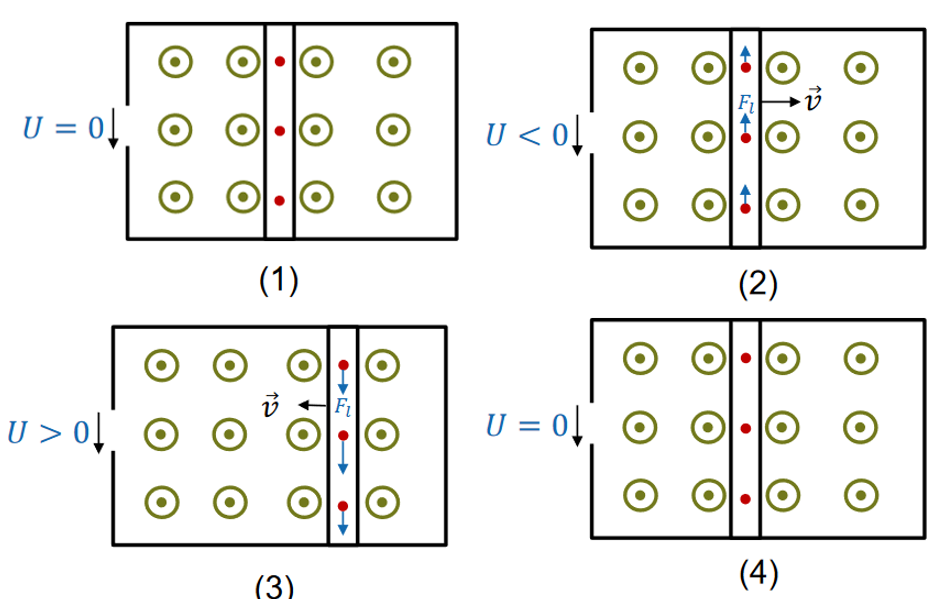
\includegraphics[scale=0.6]{img/beweg-ind} \\
    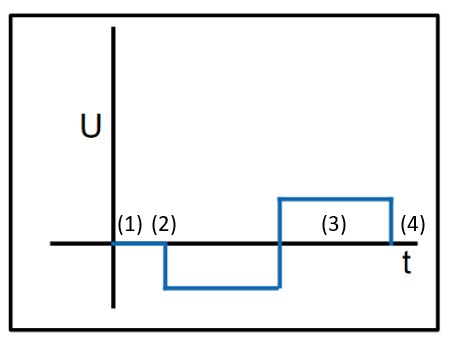
\includegraphics[scale=0.6]{img/beweg-ind-graph}
\end{center}
\definition{Bewegungsinduktion}
\beginip
Bewegen wir einen Leiter mit Lädungstrager in einem Magnetfeld, so wirkt eine magnetische Kraft auf die Ladungsträger im Leiter. \\
Die Ladungsträger werden sich desshalb in Richtung der Kraftwirkung bewegen. Diese Bewegung bezeichnen wir als \textbf{induzierter Strom}. \\

\iend

\bsptask{Beispiel}{Bewegungsinduktion}
\beginbsp
%todo
TODO
\iend

\definition{Selbstinduktion}
\beginip
%TODO
todo
\iend


\definition{Gegentinduktion}
\beginip
%TODO
todo
\iend


\subsection{Charakteristische Gleichungen von Kapazität und Induktivität}
\gl{Gleichung}{Induktivität}
\begingl
%TODO
todo
\iend

\gl{Gleichung}{Kondensator}
\begingl
Der Zusammenhang zwischen Strom und Spannung am Kondensator ist wie folgt gegeben
\formulaBegin
$\displaystyle u_c(t) = \frac{1}{C} \int_0^t i_c(t) dt$ \\

$\displaystyle i_c(t) = c \cdot \frac{d}{d t} (u_c)$ \\
\formulaEnd
\iend


\textbf{Begründung} \\
Mit dem Wissen, dass Strom definiert ist als die Ladung pro Zeit $ \displaystyle \frac{dQ}{dt} = I$ folgt folgendes: \\
\begin{center}
	$\displaystyle \frac{\partial}{\partial t} (C \cdot U) = \frac{\partial}{\partial t} (Q) $ \\
	$ \displaystyle C  \cdot \frac{dU}{dt} = I \rightarrow U(t) = \frac{1}{C} \cdot \int_0^t I \cdot dt$
\end{center}
